\subsection{Inverse DFT}

Die \gls{idft} ist die Umkehrfunktion der \gls{dft}. Wenn das Eingangssignal $x$ zeitabhängig und somit als $\vec{x}(t)$ geschrieben werden kann, dann handelt es sich bei $X$ um
dessen Darstellung im Frequenzbereich und kann als $\vec{X}(f)$ geschrieben werden. Mit der \gls{idft} ist es möglich aus der Frequendarstellung das Zeitsignal zu errechnen.
%$X(f)$ $x(t)$ 

\begin{equation}\label{eq:idft}
 x \left[ n \right] = \frac{1}{N} \sum^{N-1}_{n=0} X^*[m] \cdot e^{\frac{j 2 \pi m n}{N}}
\end{equation}

beschrieben. Durch die umgekehrte Drehrichtung des komplexen Zeigers in Gleichung (\ref{eq:idft}) werden in der Matrizenschreibweise die Zeilen 2 und 8, 3 und 7 sowie 4 und 6 vertauscht.
Nachvollziehen lässt sich das gut anhand der Grafik (\ref{pic:Einheitskreis_Faktoren}). 
Verdeutlicht wird das vorgehen in Abbildung \ref{pic:IDFT_Zeilentausch}.

\begin{figure}[ht]
 \centering
 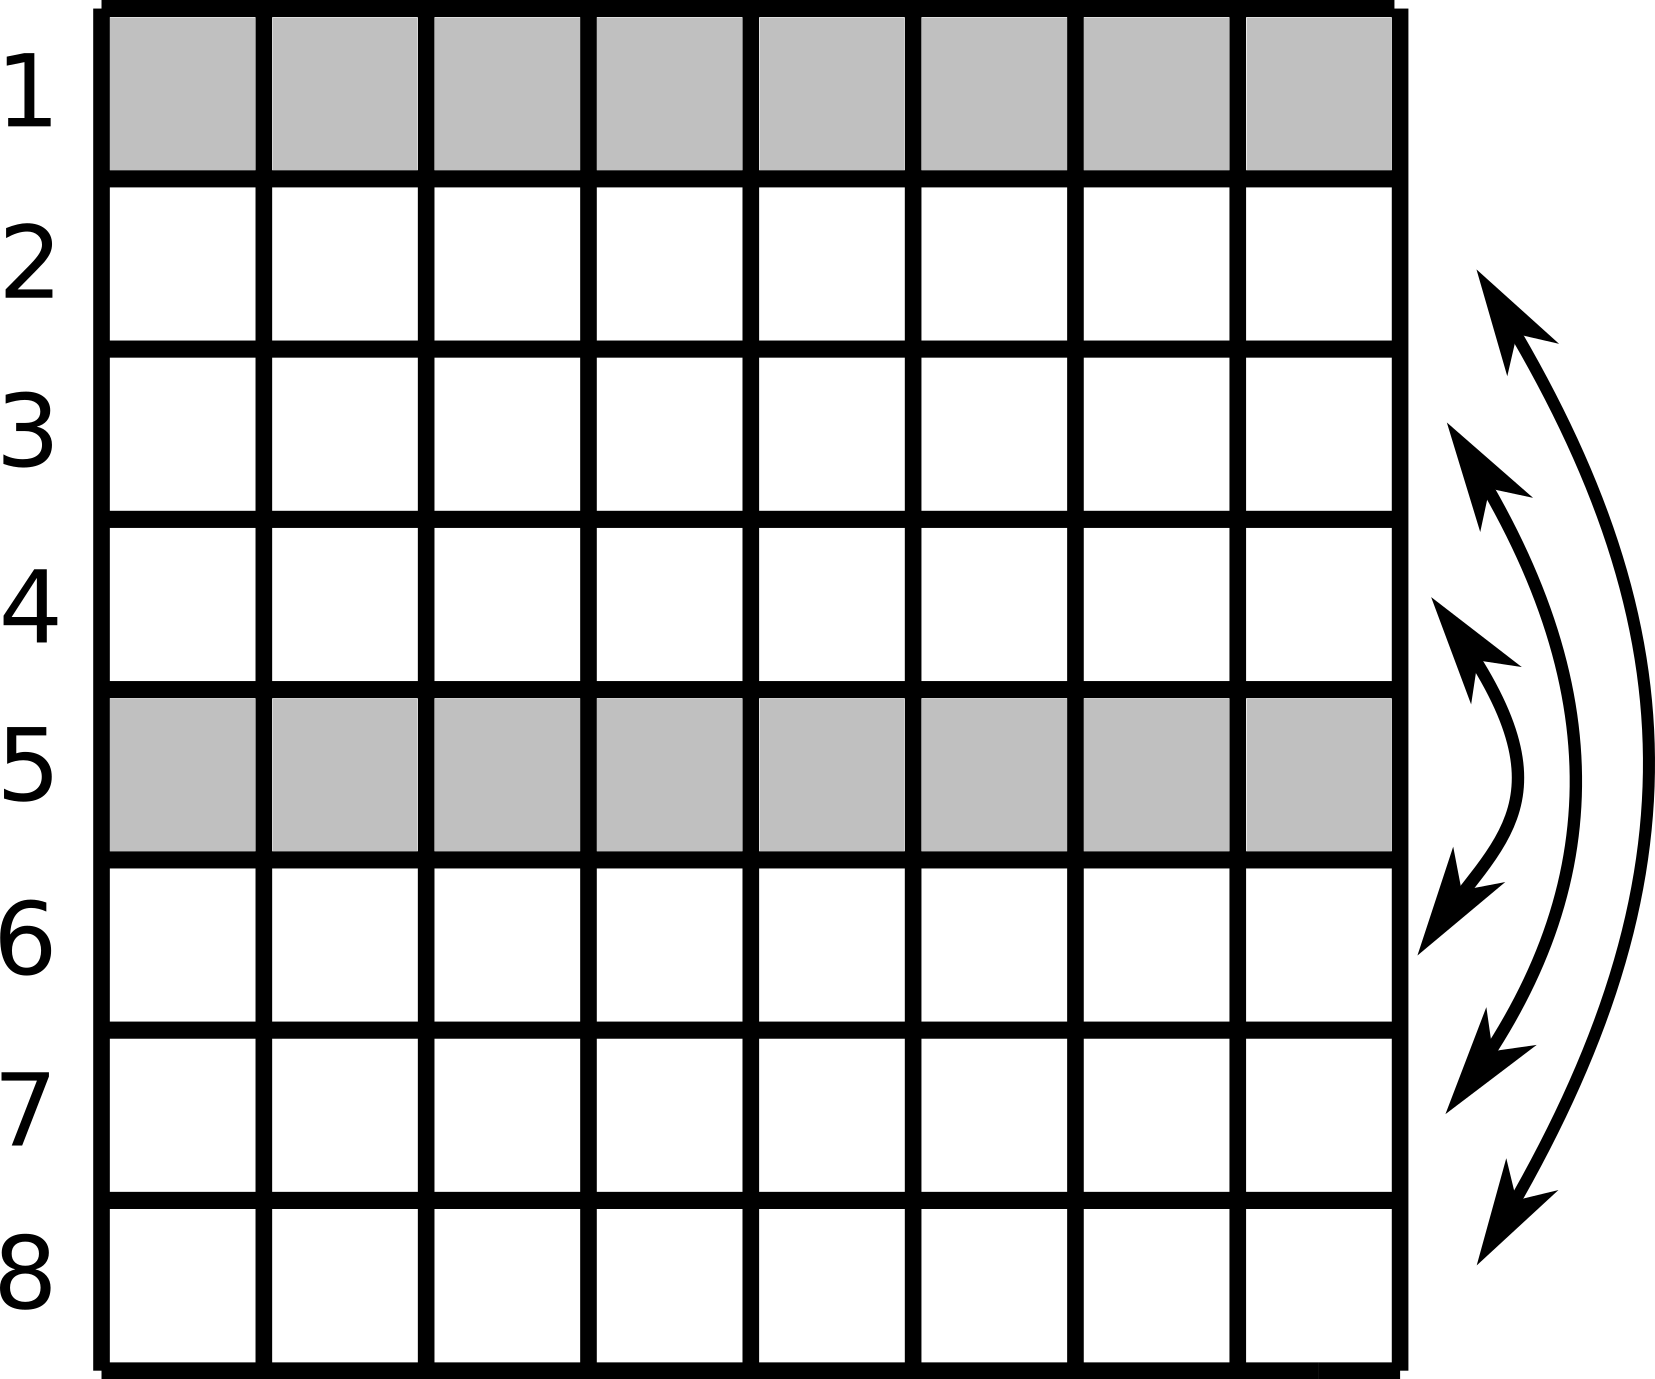
\includegraphics[width=0.4\textwidth]{img/IDFT_Zeilentausch.png}
 \caption{Um von der DFT zur IDFT zu kommen, müssen bei der Matrixmultiplikation die Zeilen der Twiddlefaktormatrix vertauscht werden}
 \label{pic:IDFT_Zeilentausch}
\end{figure}

